
\documentclass[border=8pt, multi, tikz]{standalone} 
\usepackage{import}
\subimport{../layers/}{init}
\usetikzlibrary{positioning}
\usetikzlibrary{3d} %for including external image 

\def\ConvColor{rgb:yellow,5;red,2.5;white,5}
\def\ConvReluColor{rgb:yellow,5;red,5;white,5}
\def\PoolColor{rgb:red,1;black,0.3}
\def\UnpoolColor{rgb:blue,2;green,1;black,0.3}
\def\FcColor{rgb:blue,5;red,4;white,5}
\def\FcReluColor{rgb:blue,5;red,5;white,4}
\def\SoftmaxColor{rgb:magenta,5;black,7}   
\def\SumColor{rgb:blue,5;green,15}
\def\Relu{rgb:cyan,5;green,15}
\def\Picture{rgb:blue,5;green,15}
\def\BatchNorm{rgb:pink,5;green,15}
\def\DropoutColor{rgb:magenta,5;black,7}  
\def\LSTMColor{rgb:red,5;black,3}  

\newcommand{\copymidarrow}{\tikz \draw[-Stealth,line width=0.8mm,draw={rgb:blue,4;red,1;green,1;black,3}] (-0.3,0) -- ++(0.3,0);}

\begin{document}
\begin{tikzpicture}
\tikzstyle{connection}=[ultra thick,every node/.style={sloped,allow upside down},draw=\edgecolor,opacity=0.7]
\tikzstyle{copyconnection}=[ultra thick,every node/.style={sloped,allow upside down},draw={rgb:blue,4;red,1;green,1;black,3},opacity=0.7]

\node[canvas is zy plane at x=0] (jedanslika14) at (-3,0,0) {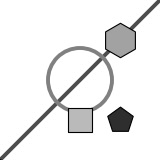
\includegraphics[width=5cm,height=5cm]{slika_1.png}};
\node[below, font=\Large] at (jedanslika14.south) {};

\pic[shift={(2,0,0)}] at (0,0,0) 
    {Box={
        name=jedanconv1,
        caption=,
        xlabel={{16, }},
        zlabel=79,
        fill=\ConvColor,
        height=19,
        width=4,
        depth=19
        }
    };

\pic[shift={(0,0,0)}] at (jedanconv1-east) 
    {Box={
        name=jedannorm1,
        caption=,
        fill=\BatchNorm,
        height=19,
        width=3,
        depth=19
        }
    };

\pic[shift={(0,0,0)}] at (jedannorm1-east) 
    {Box={
        name=jedanrelu1,
        caption=,
        fill=\Relu,
        height=19,
        width=3,
        depth=19
        }
    };

\draw [connection]  (-2, 0, 0)    -- node {\midarrow} (jedanconv1-west);

\pic[shift={(2,0,0)}] at (jedanrelu1-east) 
    {Box={
        name=jedanconv2,
        caption=,
        xlabel={{16, }},
        zlabel=38,
        fill=\ConvColor,
        height=10,
        width=4,
        depth=10
        }
    };

\pic[shift={(0,0,0)}] at (jedanconv2-east) 
    {Box={
        name=jedannorm2,
        caption=,
        fill=\BatchNorm,
        height=10,
        width=3,
        depth=10
        }
    };

\pic[shift={(0,0,0)}] at (jedannorm2-east) 
    {Box={
        name=jedanrelu2,
        caption=,
        fill=\Relu,
        height=10,
        width=3,
        depth=10
        }
    };

\draw [connection]  (jedanrelu1-east)    -- node {\midarrow} (jedanconv2-west);

\pic[shift={(2,0,0)}] at (jedanrelu2-east) 
    {Box={
        name=jedanconv3,
        caption=,
        xlabel={{16, }},
        zlabel=18,
        fill=\ConvColor,
        height=5,
        width=4,
        depth=5
        }
    };

\pic[shift={(0,0,0)}] at (jedanconv3-east) 
    {Box={
        name=jedannorm3,
        caption=,
        fill=\BatchNorm,
        height=5,
        width=3,
        depth=5
        }
    };

\pic[shift={(0,0,0)}] at (jedannorm3-east) 
    {Box={
        name=jedanrelu3,
        caption=,
        fill=\Relu,
        height=5,
        width=3,
        depth=5
        }
    };

\draw [connection]  (jedanrelu2-east)    -- node {\midarrow} (jedanconv3-west);

\pic[shift={(2,0,0)}] at (jedanrelu3-east) 
    {Box={
        name=jedanconv4,
        caption=,
        xlabel={{16, }},
        zlabel=9,
        fill=\ConvColor,
        height=2,
        width=4,
        depth=2
        }
    };

\pic[shift={(0,0,0)}] at (jedanconv4-east) 
    {Box={
        name=jedannorm4,
        caption=,
        fill=\BatchNorm,
        height=2,
        width=3,
        depth=2
        }
    };

\pic[shift={(0,0,0)}] at (jedannorm4-east) 
    {Box={
        name=jedanrelu4,
        caption=,
        fill=\Relu,
        height=2,
        width=3,
        depth=2
        }
    };

\draw [connection]  (jedanrelu3-east)    -- node {\midarrow} (jedanconv4-west);

\pic[shift={(2,0,0)}] at (jedanrelu4-east) 
    {Box={
        name=jedanlstm1,
        caption=,
        xlabel={{, }},
        zlabel=,
        fill=\LSTMColor,
        height=10,
        width=10,
        depth=10
        }
    };

\draw [connection]  (jedanrelu4-east)    -- node {\midarrow} (jedanlstm1-west);

\node[canvas is zy plane at x=0] (dvaslika14) at (-3,10,0) {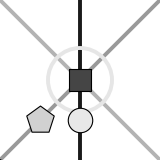
\includegraphics[width=5cm,height=5cm]{slika_2.png}};
\node[below, font=\Large] at (dvaslika14.south) {};

\pic[shift={(2,10,0)}] at (0,0,0) 
    {Box={
        name=dvaconv1,
        caption=,
        xlabel={{16, }},
        zlabel=79,
        fill=\ConvColor,
        height=19,
        width=4,
        depth=19
        }
    };

\pic[shift={(0,0,0)}] at (dvaconv1-east) 
    {Box={
        name=dvanorm1,
        caption=,
        fill=\BatchNorm,
        height=19,
        width=3,
        depth=19
        }
    };

\pic[shift={(0,0,0)}] at (dvanorm1-east) 
    {Box={
        name=dvarelu1,
        caption=,
        fill=\Relu,
        height=19,
        width=3,
        depth=19
        }
    };

\draw [connection]  (-2, 10, 0)    -- node {\midarrow} (dvaconv1-west);

\pic[shift={(2,0,0)}] at (dvarelu1-east) 
    {Box={
        name=dvaconv2,
        caption=,
        xlabel={{16, }},
        zlabel=38,
        fill=\ConvColor,
        height=10,
        width=4,
        depth=10
        }
    };

\pic[shift={(0,0,0)}] at (dvaconv2-east) 
    {Box={
        name=dvanorm2,
        caption=,
        fill=\BatchNorm,
        height=10,
        width=3,
        depth=10
        }
    };

\pic[shift={(0,0,0)}] at (dvanorm2-east) 
    {Box={
        name=dvarelu2,
        caption=,
        fill=\Relu,
        height=10,
        width=3,
        depth=10
        }
    };

\draw [connection]  (dvarelu1-east)    -- node {\midarrow} (dvaconv2-west);

\pic[shift={(2,0,0)}] at (dvarelu2-east) 
    {Box={
        name=dvaconv3,
        caption=,
        xlabel={{16, }},
        zlabel=18,
        fill=\ConvColor,
        height=5,
        width=4,
        depth=5
        }
    };

\pic[shift={(0,0,0)}] at (dvaconv3-east) 
    {Box={
        name=dvanorm3,
        caption=,
        fill=\BatchNorm,
        height=5,
        width=3,
        depth=5
        }
    };

\pic[shift={(0,0,0)}] at (dvanorm3-east) 
    {Box={
        name=dvarelu3,
        caption=,
        fill=\Relu,
        height=5,
        width=3,
        depth=5
        }
    };

\draw [connection]  (dvarelu2-east)    -- node {\midarrow} (dvaconv3-west);

\pic[shift={(2,0,0)}] at (dvarelu3-east) 
    {Box={
        name=dvaconv4,
        caption=,
        xlabel={{16, }},
        zlabel=9,
        fill=\ConvColor,
        height=2,
        width=4,
        depth=2
        }
    };

\pic[shift={(0,0,0)}] at (dvaconv4-east) 
    {Box={
        name=dvanorm4,
        caption=,
        fill=\BatchNorm,
        height=2,
        width=3,
        depth=2
        }
    };

\pic[shift={(0,0,0)}] at (dvanorm4-east) 
    {Box={
        name=dvarelu4,
        caption=,
        fill=\Relu,
        height=2,
        width=3,
        depth=2
        }
    };

\draw [connection]  (dvarelu3-east)    -- node {\midarrow} (dvaconv4-west);

\pic[shift={(2,0,0)}] at (dvarelu4-east) 
    {Box={
        name=dvalstm1,
        caption=,
        xlabel={{, }},
        zlabel=,
        fill=\LSTMColor,
        height=10,
        width=10,
        depth=10
        }
    };

\draw [connection]  (dvarelu4-east)    -- node {\midarrow} (dvalstm1-west);

\draw [connection]  (dvalstm1-east)    -- node {\midarrow} (jedanlstm1-east);

\draw [connection]  (dvalstm1-south)    -- node {\midarrow} (jedanlstm1-north);
\filldraw[fill=black] (0,0) ++(3,4) circle (0.1);
            \filldraw[fill=black] (0,1) ++(3,4) circle (0.1);
            \filldraw[fill=black] (0,2) ++(3,4) circle (0.1);
            \filldraw[fill=black] (0,0) ++(18,4) circle (0.1);
            \filldraw[fill=black] (0,1) ++(18,4) circle (0.1);
            \filldraw[fill=black] (0,2) ++(18,4) circle (0.1);
            
\pic[shift={(4,-2,0)}] at (jedanlstm1-south) 
    {Box={
        name=Dropout,
        caption=\\,
        fill=\DropoutColor,
        height=50,
        width=3,
        depth=3
        }
    };

\pic[shift={(0,0,0)}] at (Dropout-east) 
    {Box={
        name=linear3,
        caption=,
        zlabel=96,
        fill=\FcColor,
        height=50,
        width=3,
        depth=3
        }
    };

\draw [connection]  (jedanlstm1-south)    |- node {\midarrow} (Dropout-west);

\pic[shift={(4,0,0)}] at (linear3-east) 
    {Box={
        name=linear4,
        caption=,
        zlabel=8,
        fill=\FcColor,
        height=25,
        width=3,
        depth=3
        }
    };

\draw [connection]  (linear3-east)    -- node {\midarrow} (linear4-west);

\fill[white] (33,13) rectangle ++(-12,-4);
\draw (33,13) rectangle ++(-12,-4);

\filldraw[fill=\ConvColor] (22,12) ++(-0.5,0) circle (0.2);
\node[font=\Large, anchor=west] at (22,12) {\textcolor{black}{Konvolucija (3x3)}};

\filldraw[fill=\BatchNorm] (22,11) ++(-0.5,0) circle (0.2);
\node[font=\Large, anchor=west] at (22,11) {\textcolor{black}{Normalizacija Grupe}};

\filldraw[fill=\Relu] (22,10) ++(-0.5,0) circle (0.2);
\node[font=\Large, anchor=west] at (22,10) {\textcolor{black}{ReLu funkcja}};

\filldraw[fill=\FcColor] (28,12) ++(-0.5,0) circle (0.2);
\node[font=\Large, anchor=west] at (28,12) {\textcolor{black}{Linearni sloj}};

\filldraw[fill=\DropoutColor] (28,11) ++(-0.5,0) circle (0.2);
\node[font=\Large, anchor=west] at (28,11) {\textcolor{black}{Izostavljanje(0.5)}};

\filldraw[fill=\LSTMColor] (28,10) ++(-0.5,0) circle (0.2);
\node[font=\Large, anchor=west] at (28,10) {\textcolor{black}{LSTM blok}};
    
\end{tikzpicture}
\end{document}
